\documentclass{loyola-beamer}
\renewcommand{\titlelogo}{logo/luc-rev.svg}
\renewcommand{\slidelogo}{logo/luc.svg}
\usepackage{physics}
\usepackage{graphicx}
\usepackage{hyperref}


\title{Summer Training - ICS399}
\subtitle{Software Engineer at Mawqoot}

\author{Alfaifi, Ammar}
\institute{KFUPM}
\renewcommand{\slidefoot}{Department of Information \& Computer Science}

\begin{document}

\begin{titleframe}{}
	\maketitle
\end{titleframe}

\begin{frame}{Contents}
	\tableofcontents
\end{frame}


% Start of the slides

\section{About Me}

\begin{frame}{About me :)}
	I'm Ammar Alfaifi, senior student. Some work I've done
	\vspace{\baselineskip}

	\begin{itemize}
		\item Double major in Physics and Computer science.
		\item Simulation and physics numerical solutions.
		\item ML and AI models: Weather status predictor.
		      \href{https://github.com/ammar-faifi/Weather\_Status\_Predictor\_From\_Images}{\underline{Repo}}
		\item Worked on many \texttt{djagno} projects, GraphQL/REST API. \href{https://Petroly.co/}{\underline{Petroly.co}}
	\end{itemize}

\end{frame}

\begin{titleframe}{Company and Product}
	Info about the company and its main product
\end{titleframe}

% New slide
\section{Mawqoot and Its Company}

\begin{frame}{Company Info}
	\textbf{Vision:} Our vision is to be at the forefront of pioneering technological advancements.
	We harness modern technologies to serve various sectors, making them accessible to all
	\vspace{\baselineskip}

	\begin{itemize}
		\item Sanim Information Technology.
		\item located in the Dhahran Techno Valley at KFUPM.
	\end{itemize}
\end{frame}


% New slide
\section{Company's Main Product}

\begin{frame}{Mawqoot}
	\begin{itemize}
		\item Empowers employees with self-service capabilities.
		\item Streamlines operations by replacing paper records and spreadsheets.
		\item Mawqoot presents a cloud-based solution redefining personnel management.
		\item Fusion of mobile apps and a web platform for overseeing attendance, leave, and payroll.
	\end{itemize}
\end{frame}

\begin{frame}{Attendance Management}
	\begin{itemize}
		\item Core: Robust attendance management.
		\item Access to attendance timesheet for corrections.
		\item App features: Location tracking, biometric verification.
		\item Tracks daily attendance, identifies tardiness, departures, and absences.
	\end{itemize}
\end{frame}

\begin{frame}{Compliance and Performance}
	\begin{itemize}
		\item Enhances compliance, provides insights for decisions.
		\item Automated system detects employee infractions, enforces penalties.
	\end{itemize}
\end{frame}

\begin{frame}{Leave and Payroll Management}
	\begin{itemize}
		\item Revolutionizes leave and payroll procedures.
		\item Employees request leave, access annual leave balance.
		\item System deducts leave from salaries, managers approve requests.
		\item Administrators generate detailed payrolls, comprehensive payslips.
		\item Simplifies leave requests, payroll generation; eliminates paper workflows.
	\end{itemize}
\end{frame}

\begin{frame}{Mawqoot Inteface}
	\begin{figure}
		\begin{center}
			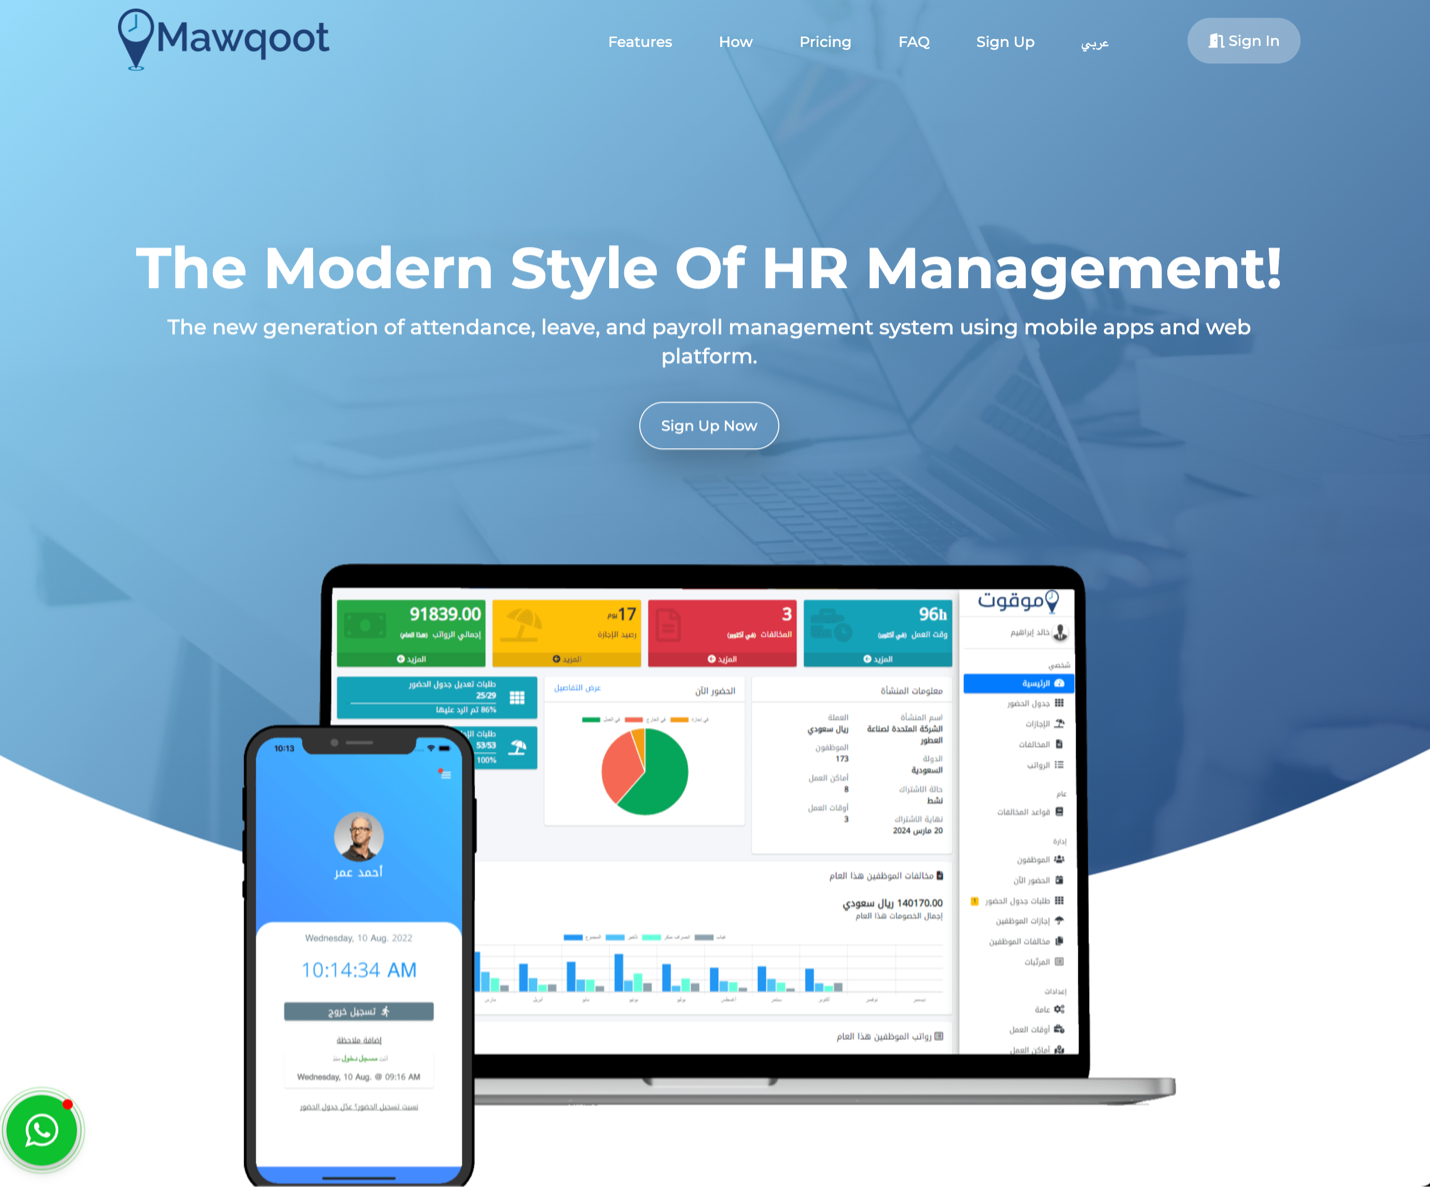
\includegraphics[width=0.5\textwidth]{figures/site.png}
		\end{center}
		\caption{The Mawqoot main site, showing the UI.}
	\end{figure}
\end{frame}

\begin{frame}{Mawqoot Inteface}
	\begin{figure}
		\begin{center}
			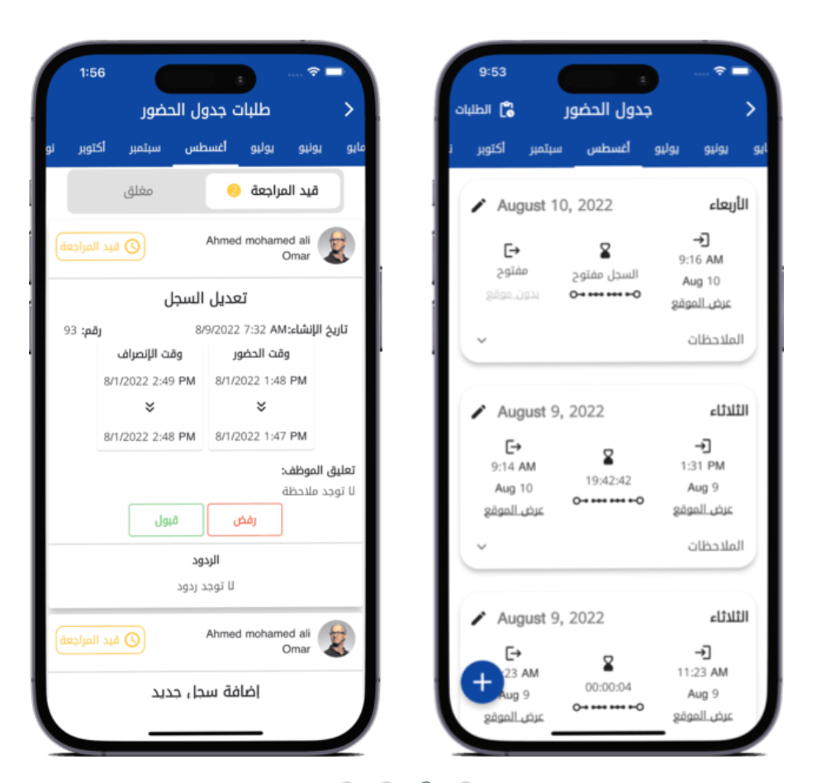
\includegraphics[width=0.45\textwidth]{figures/mobile.png}
		\end{center}
		\caption{A show case for the mobile app.}
	\end{figure}
\end{frame}


% ----- Work experience ------- %

\begin{titleframe}{Work Experience}
	Projects and features I worked on during my trainging.
\end{titleframe}

% New Section
\section{Request Petition Feature}

\begin{frame}{Request Petition}
	To allow an employee to request a petition to cancel an offence he/she has.

	\begin{figure}
		\begin{center}
			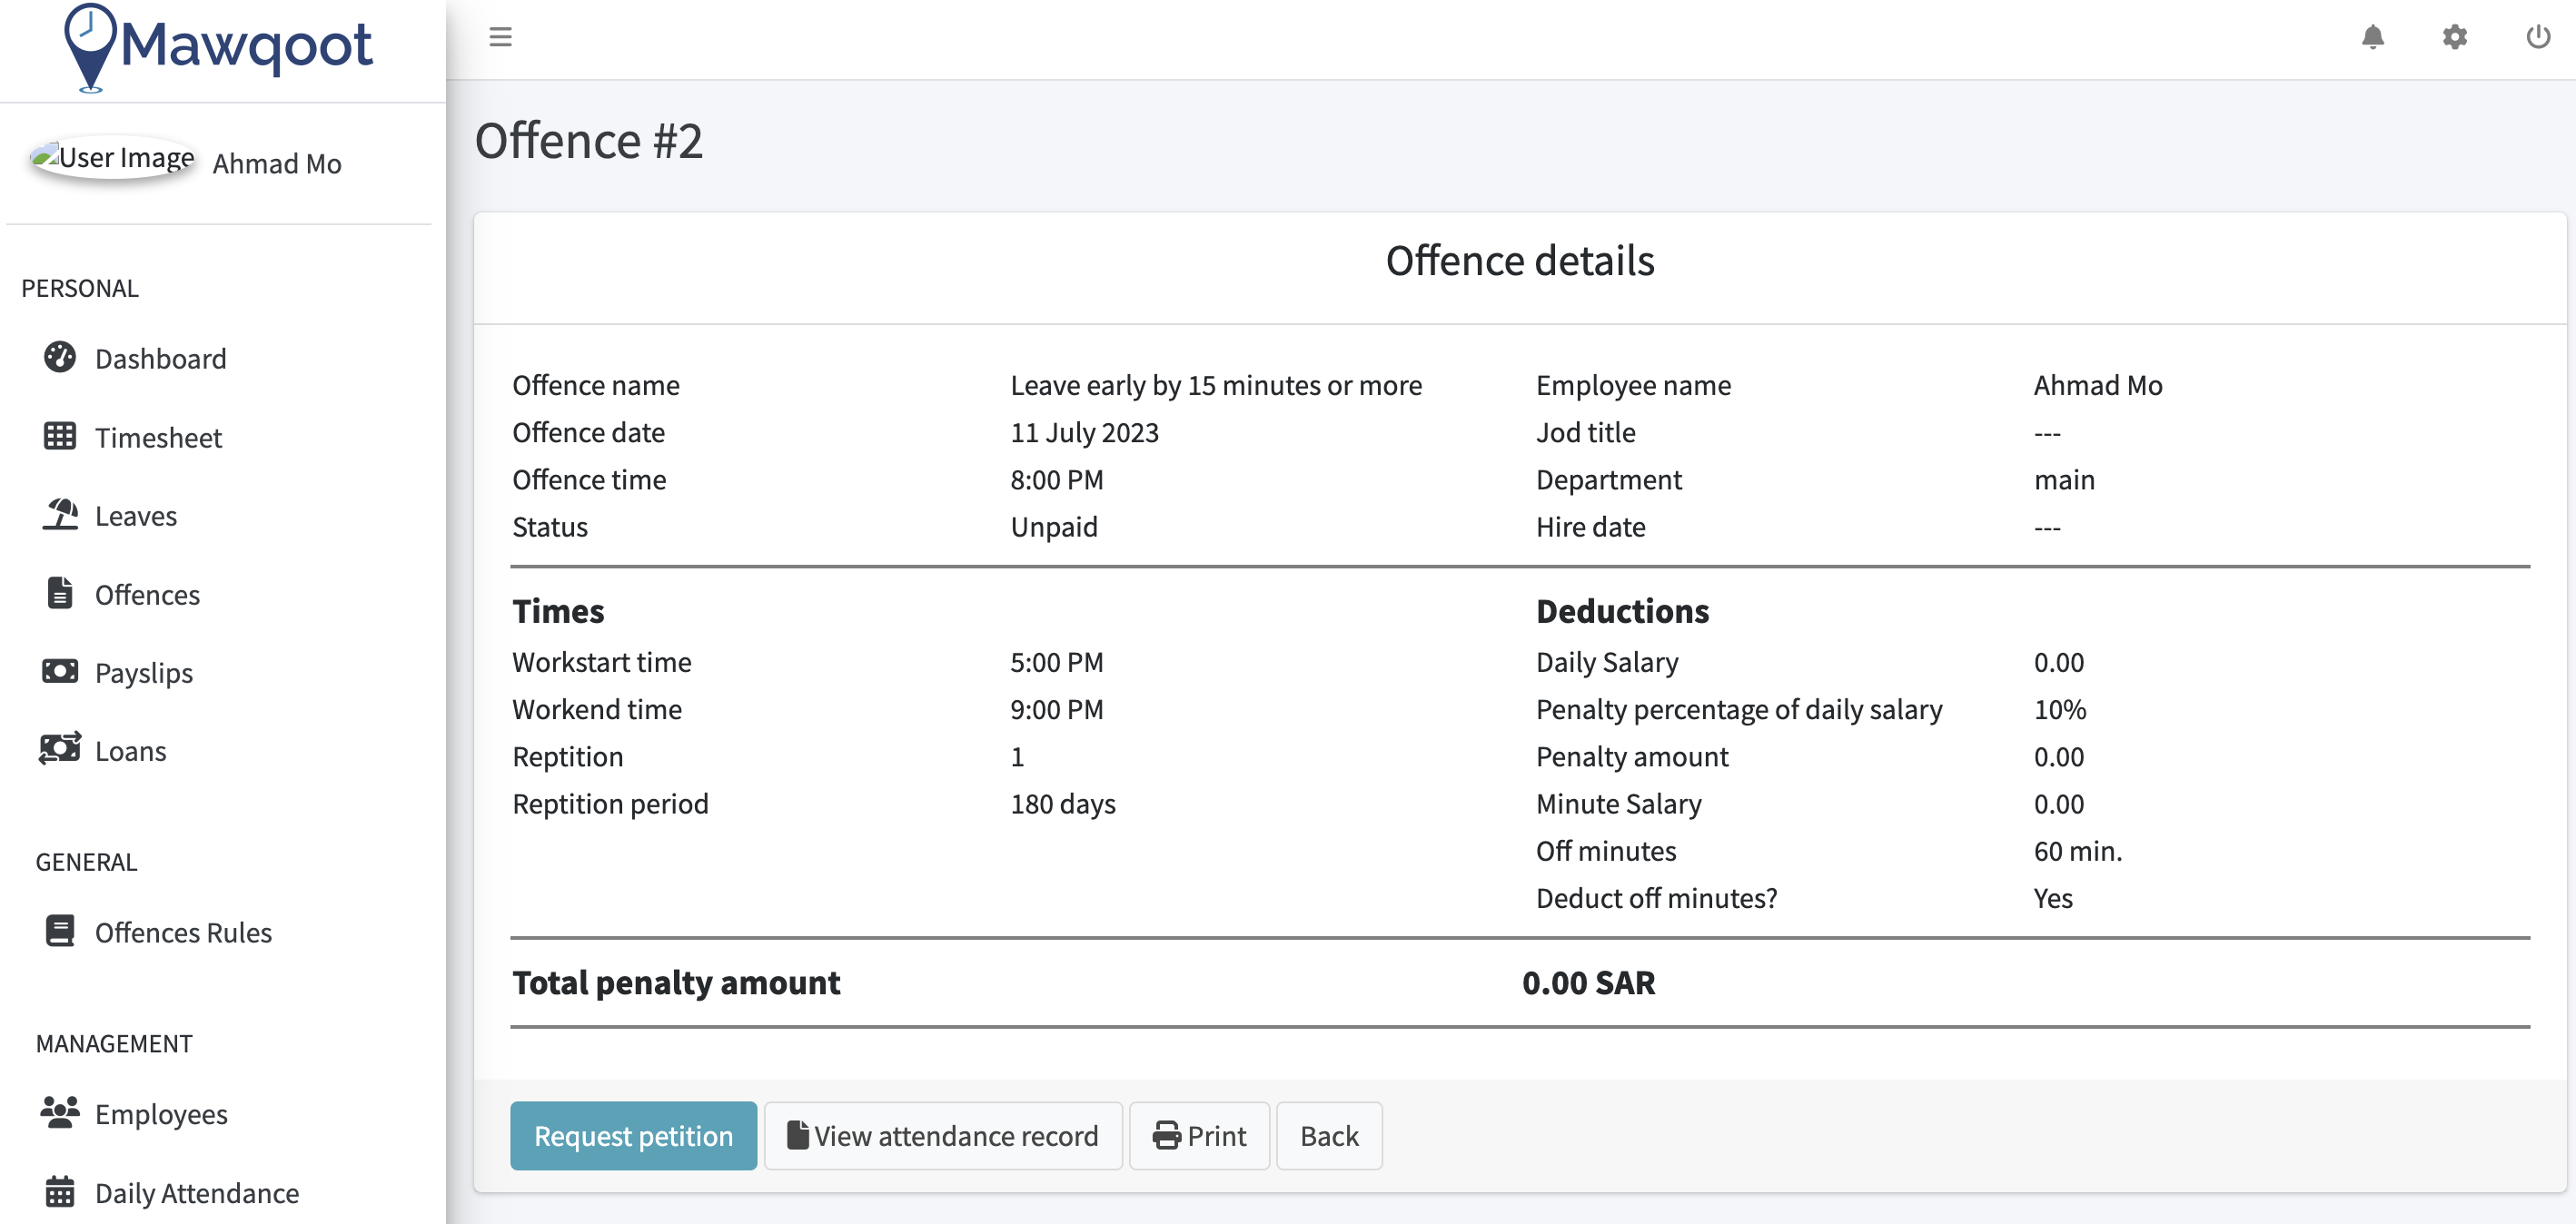
\includegraphics[width=0.7\textwidth]{figures/offence.png}
		\end{center}
		\caption{An example of offence that'll be deducted from next salary.}
	\end{figure}
\end{frame}

\begin{frame}{Request Petition}
	\begin{figure}
		\begin{center}
			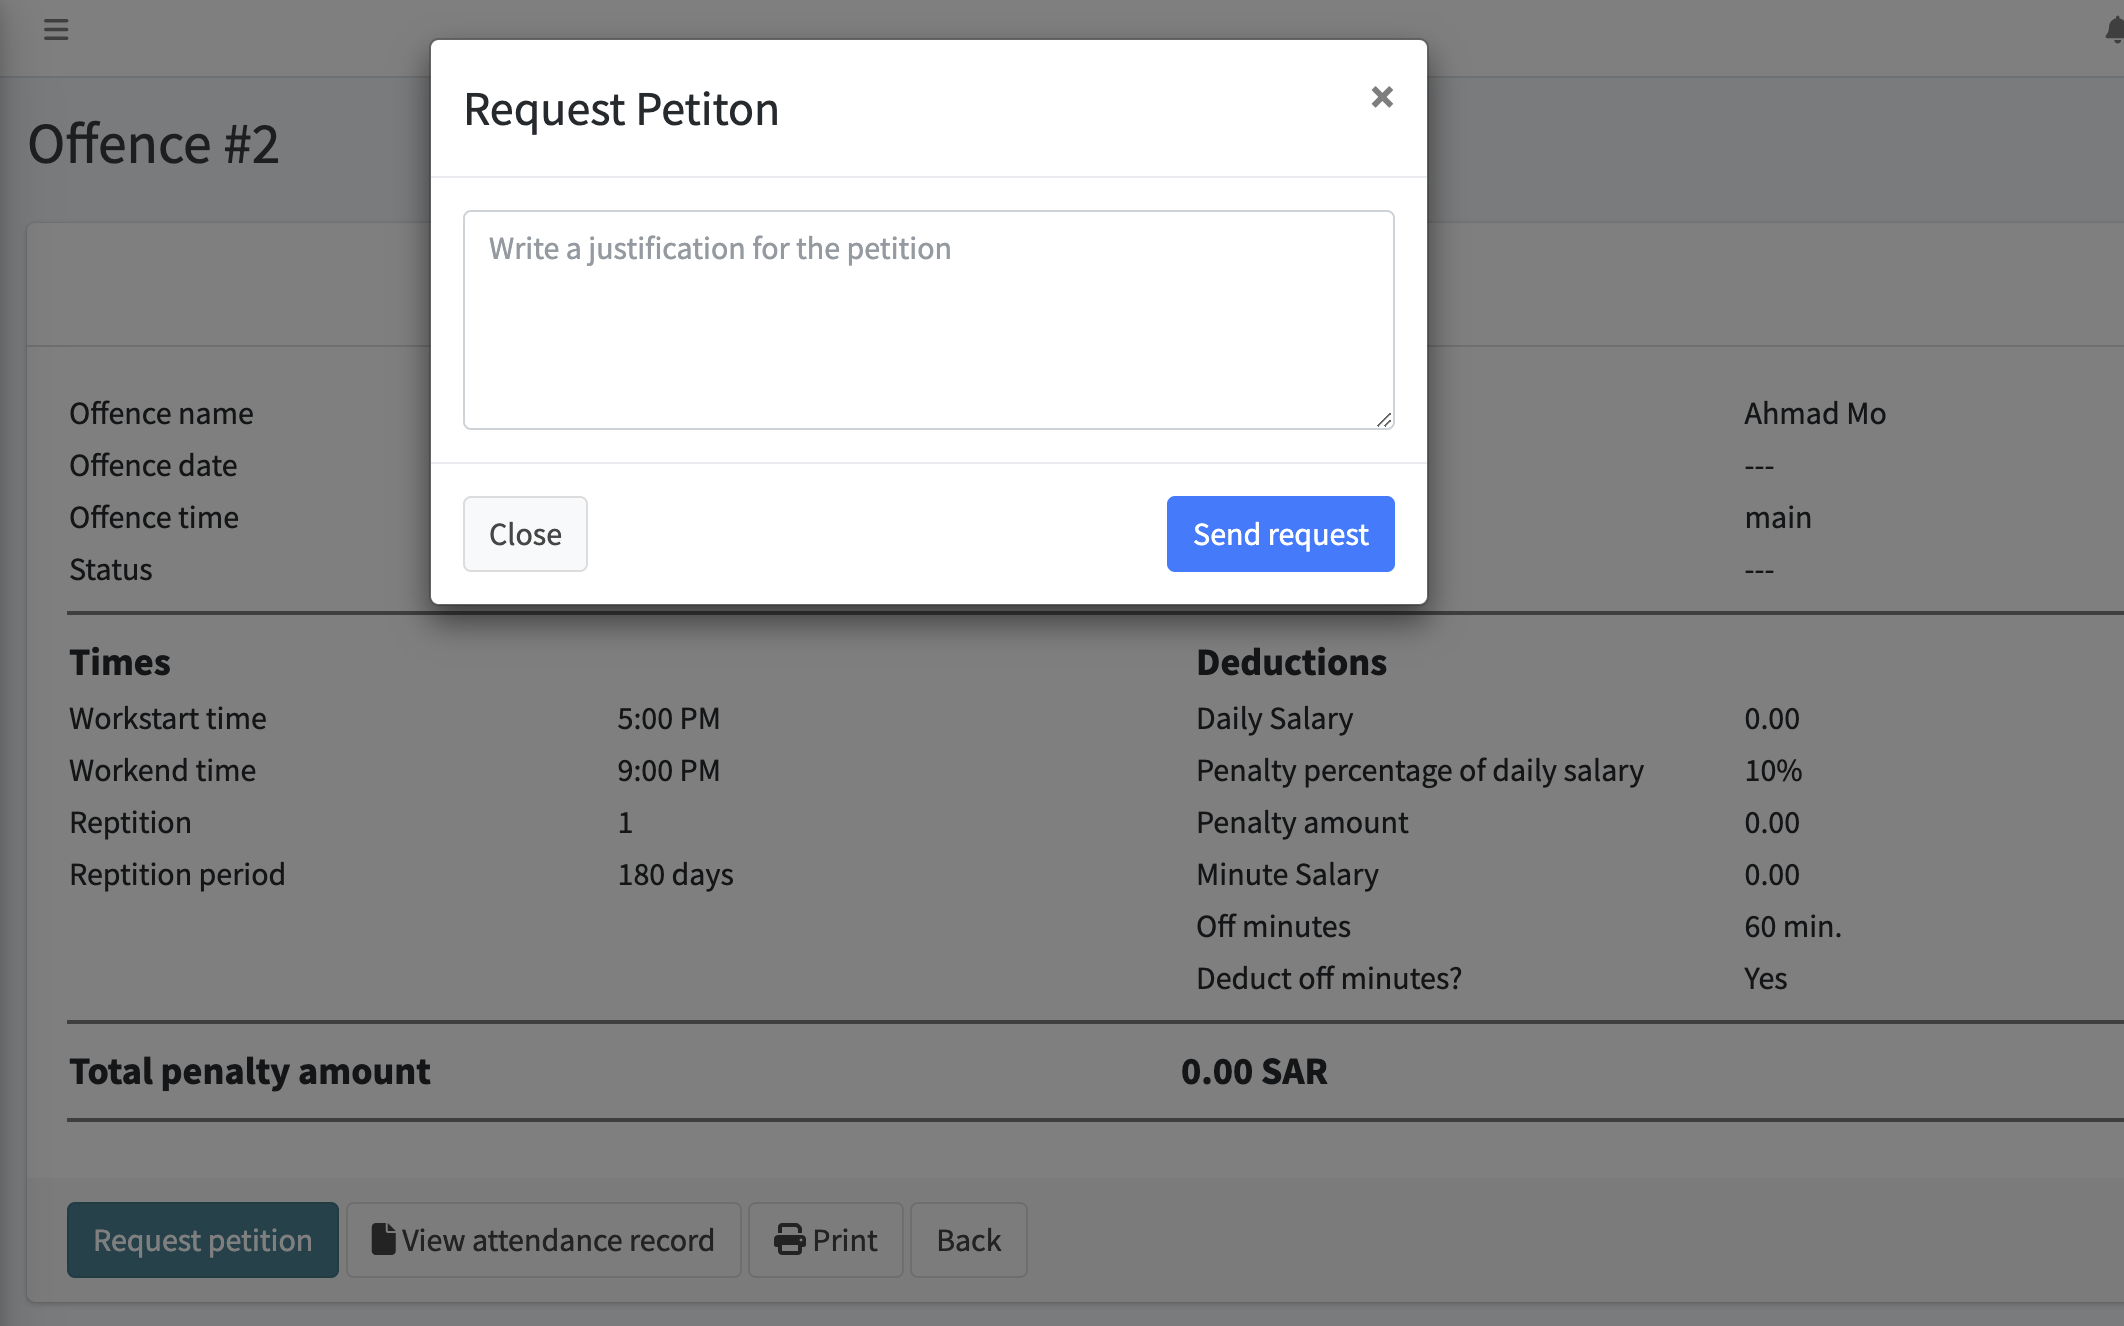
\includegraphics[width=0.7\textwidth]{figures/petition-body.png}
		\end{center}
		\caption{Employee writes why this offence should be cancelled.}
	\end{figure}
\end{frame}

\begin{frame}{Request Petition}
	\begin{figure}
		\begin{center}
			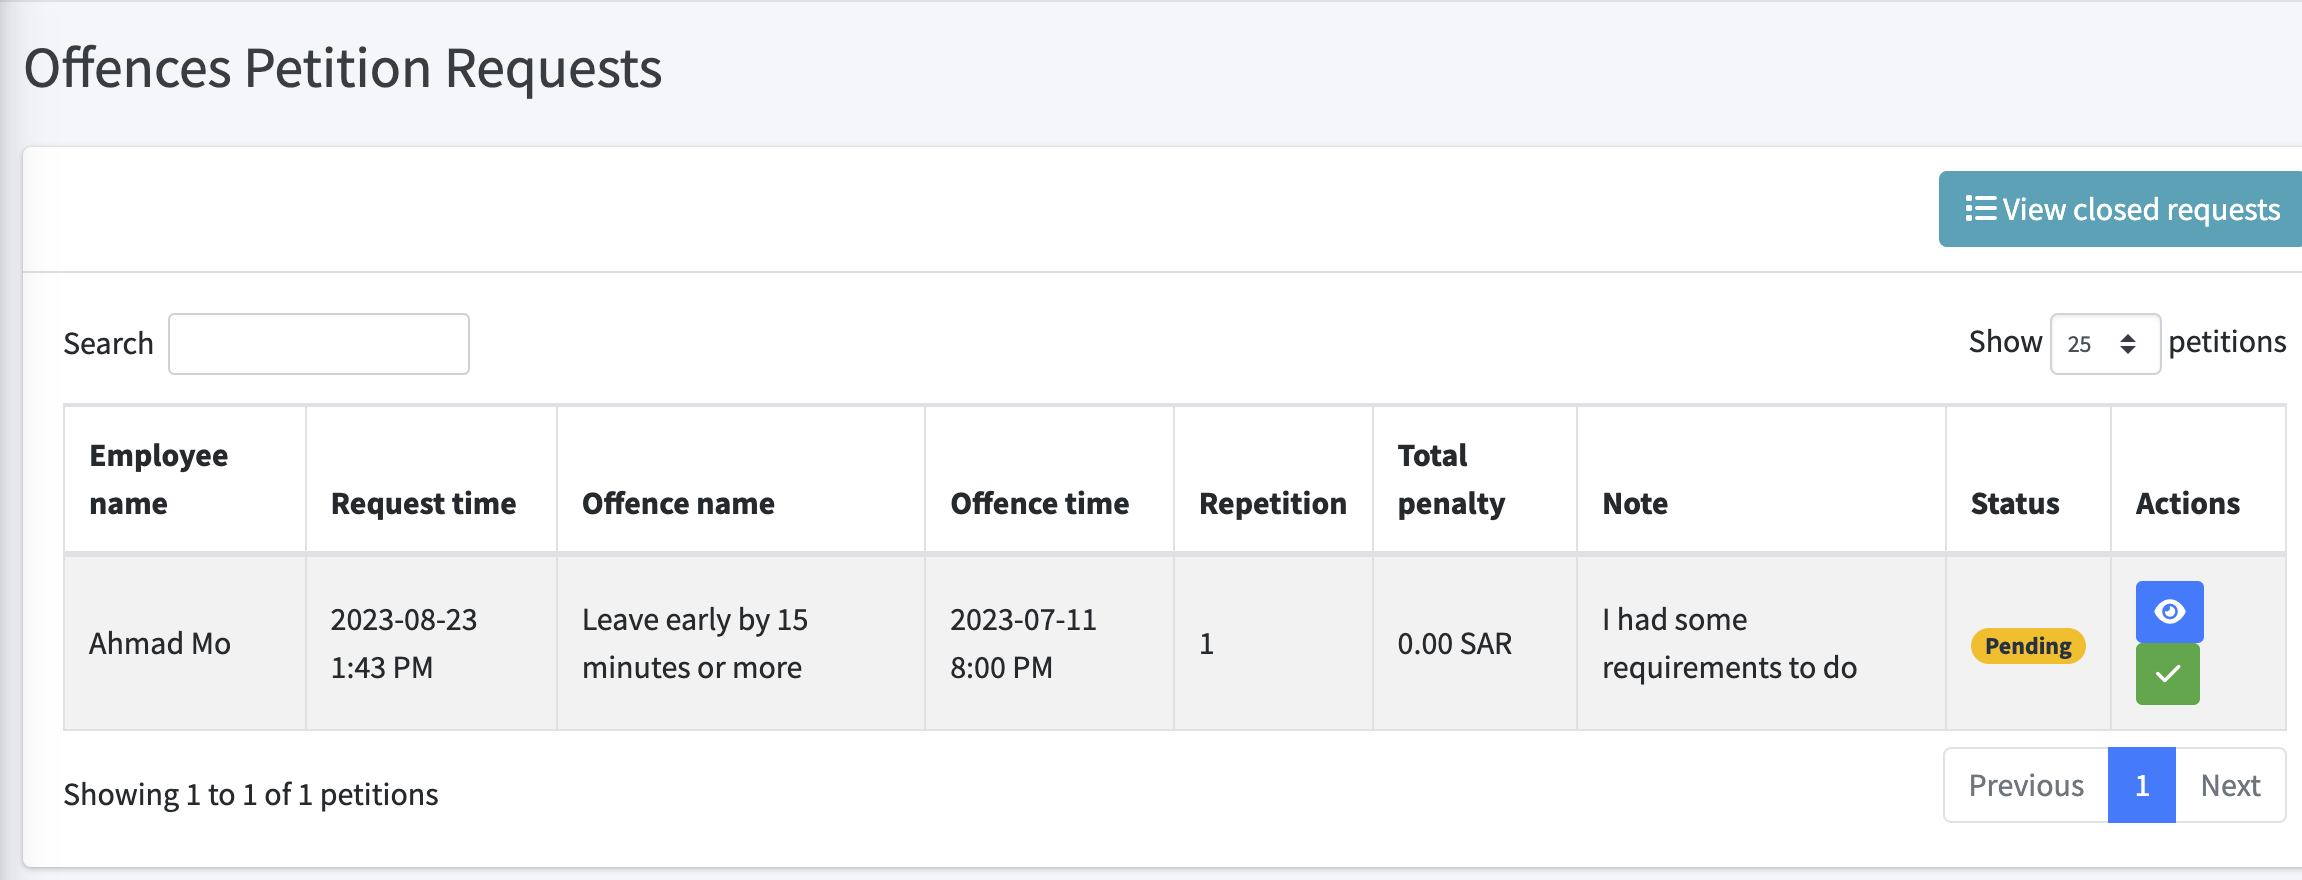
\includegraphics[width=0.9\textwidth]{figures/admin-approve.png}
		\end{center}
		\caption{All admin in approve chain needs to approve in order.}
	\end{figure}
\end{frame}

\begin{frame}{Request Petition}
	\begin{figure}
		\begin{center}
			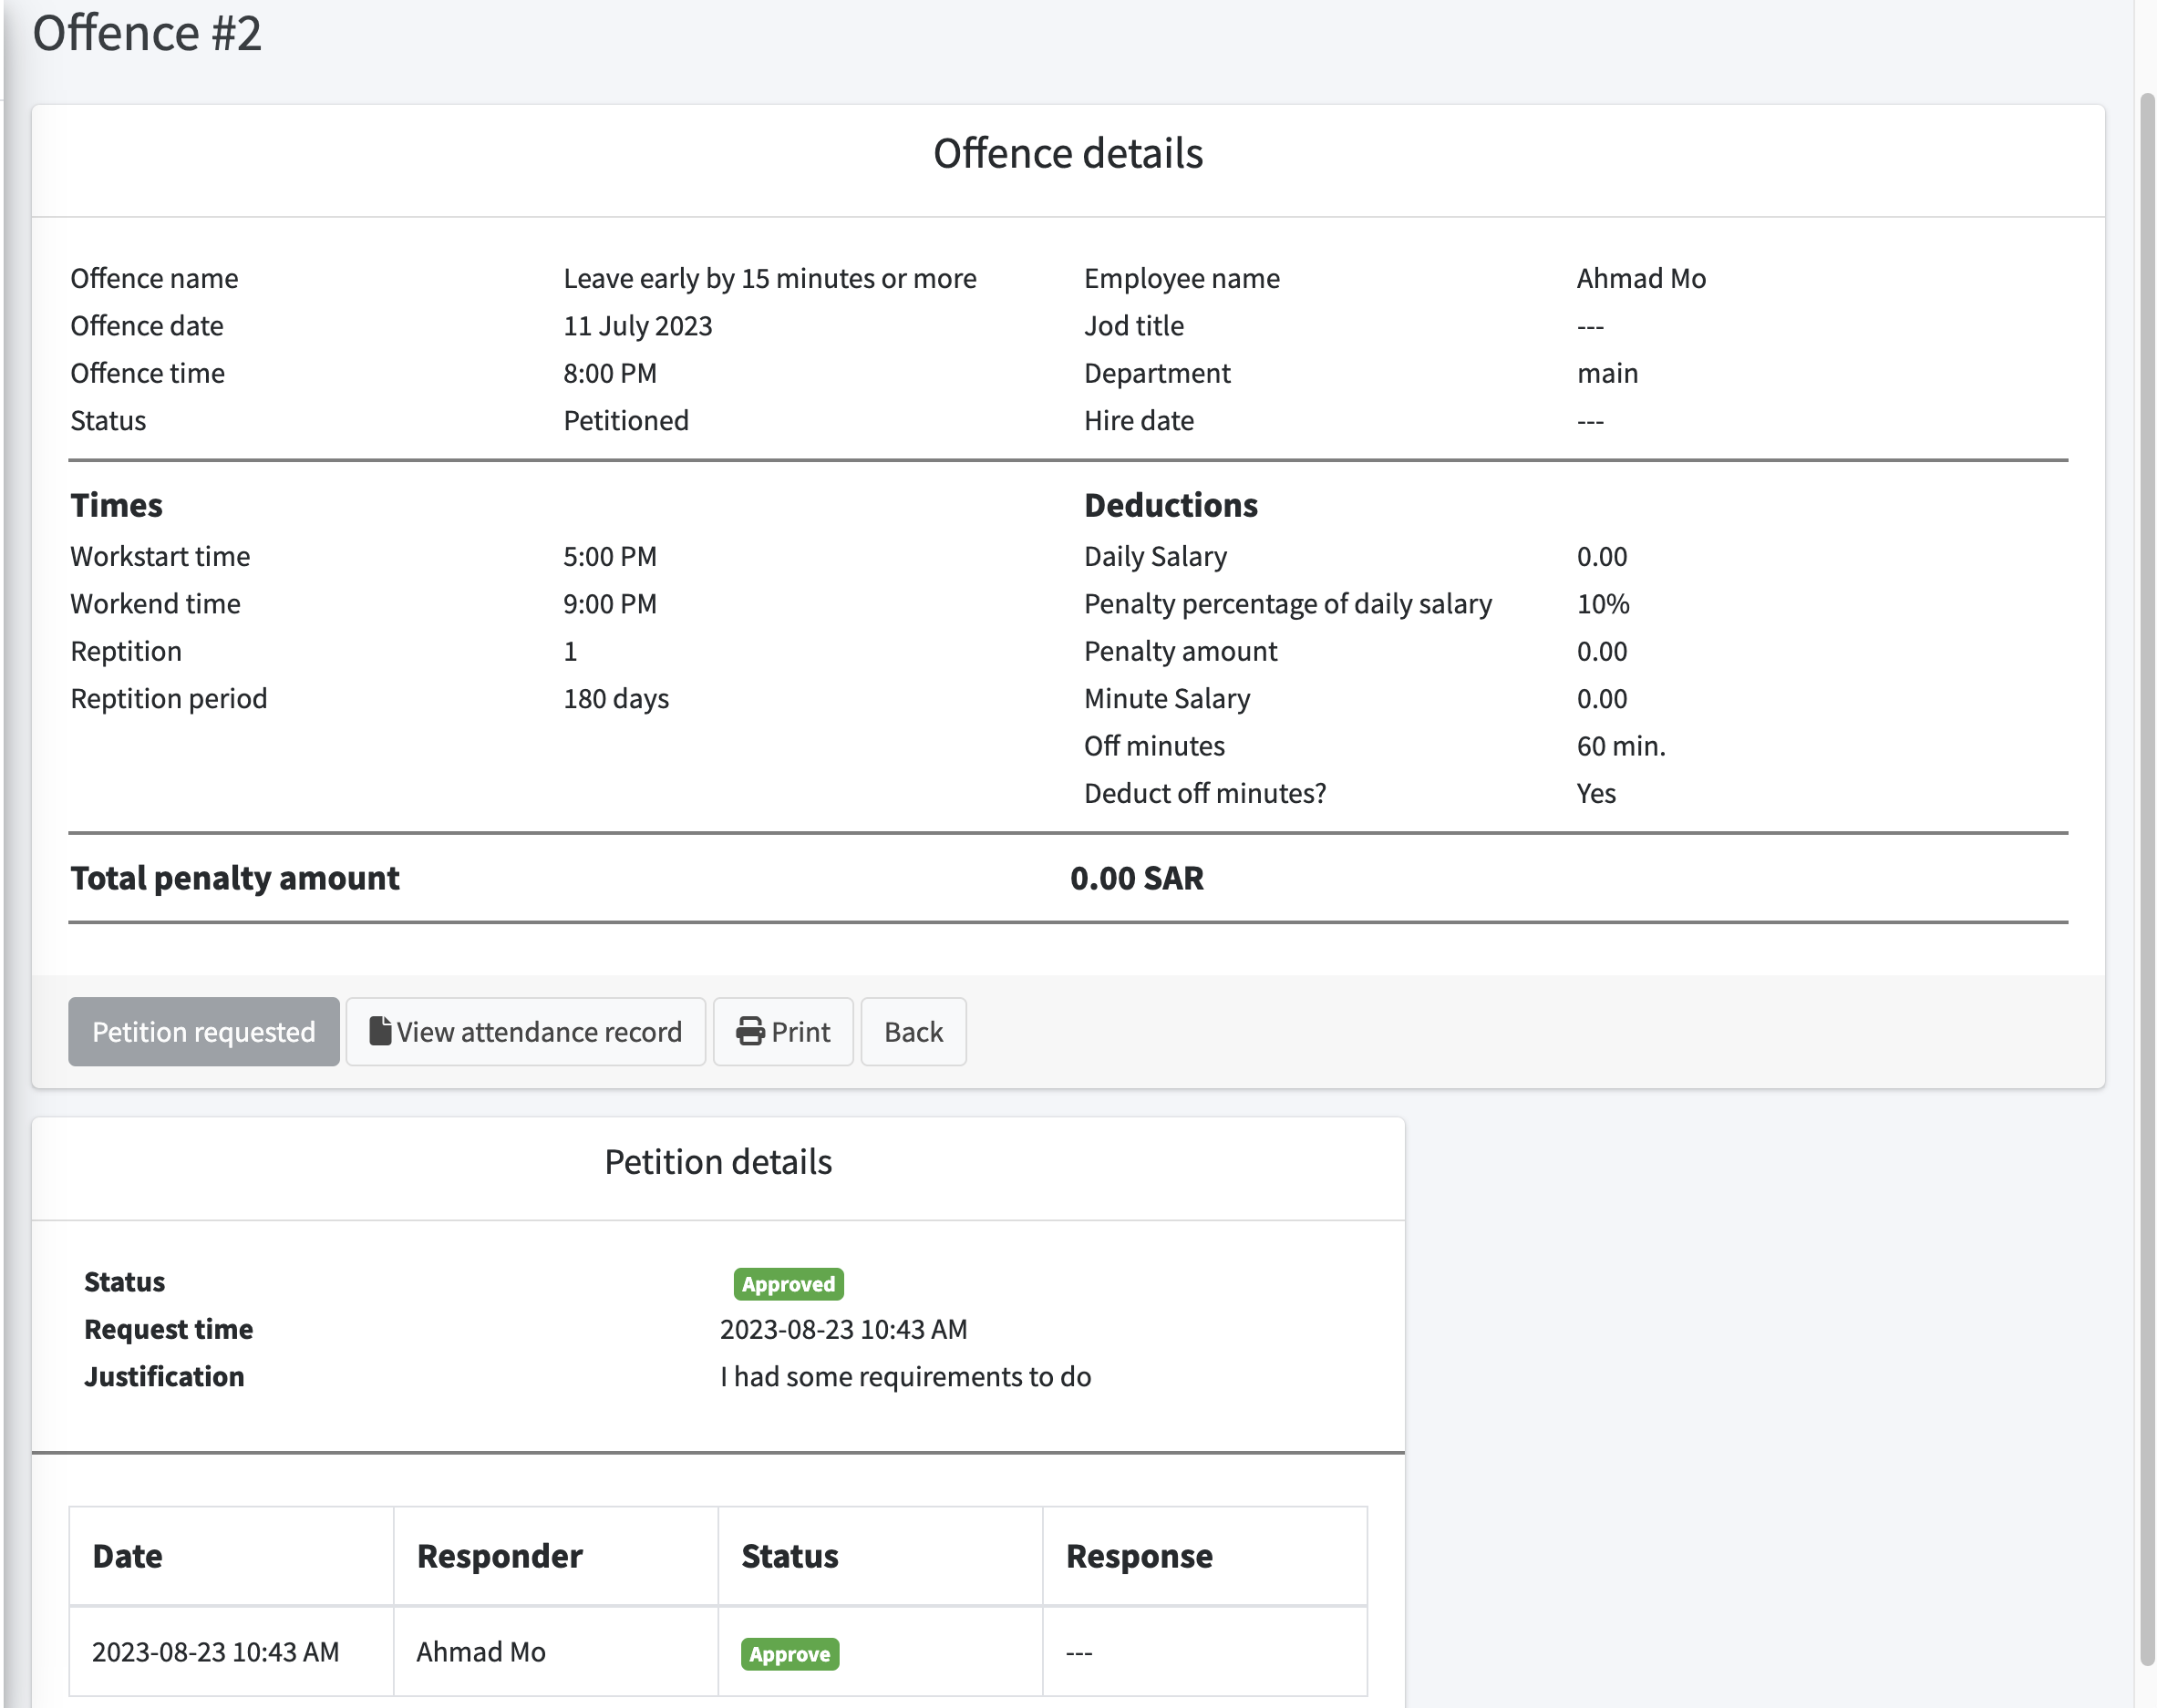
\includegraphics[width=0.55\textwidth]{figures/approved-pet.png}
		\end{center}
		\caption{An example of approved petition.}
	\end{figure}
\end{frame}

% New Section
\section{Loan Feature}

\begin{frame}{Loans Feature}
	\begin{figure}
		\begin{center}
			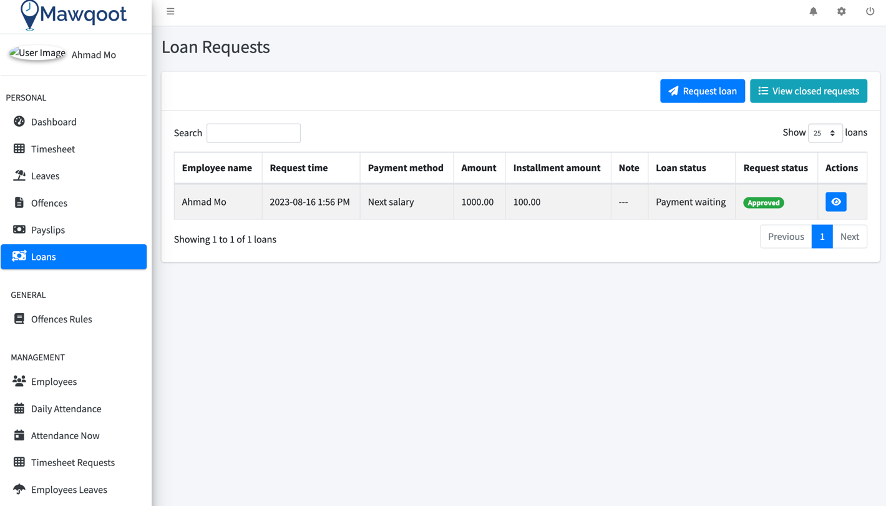
\includegraphics[width=0.7\textwidth]{figures/loans.png}
		\end{center}
		\caption{A detailed list showing employee's active loans.}
	\end{figure}
\end{frame}

\begin{frame}{Loans Feature}
	\begin{figure}
		\begin{center}
			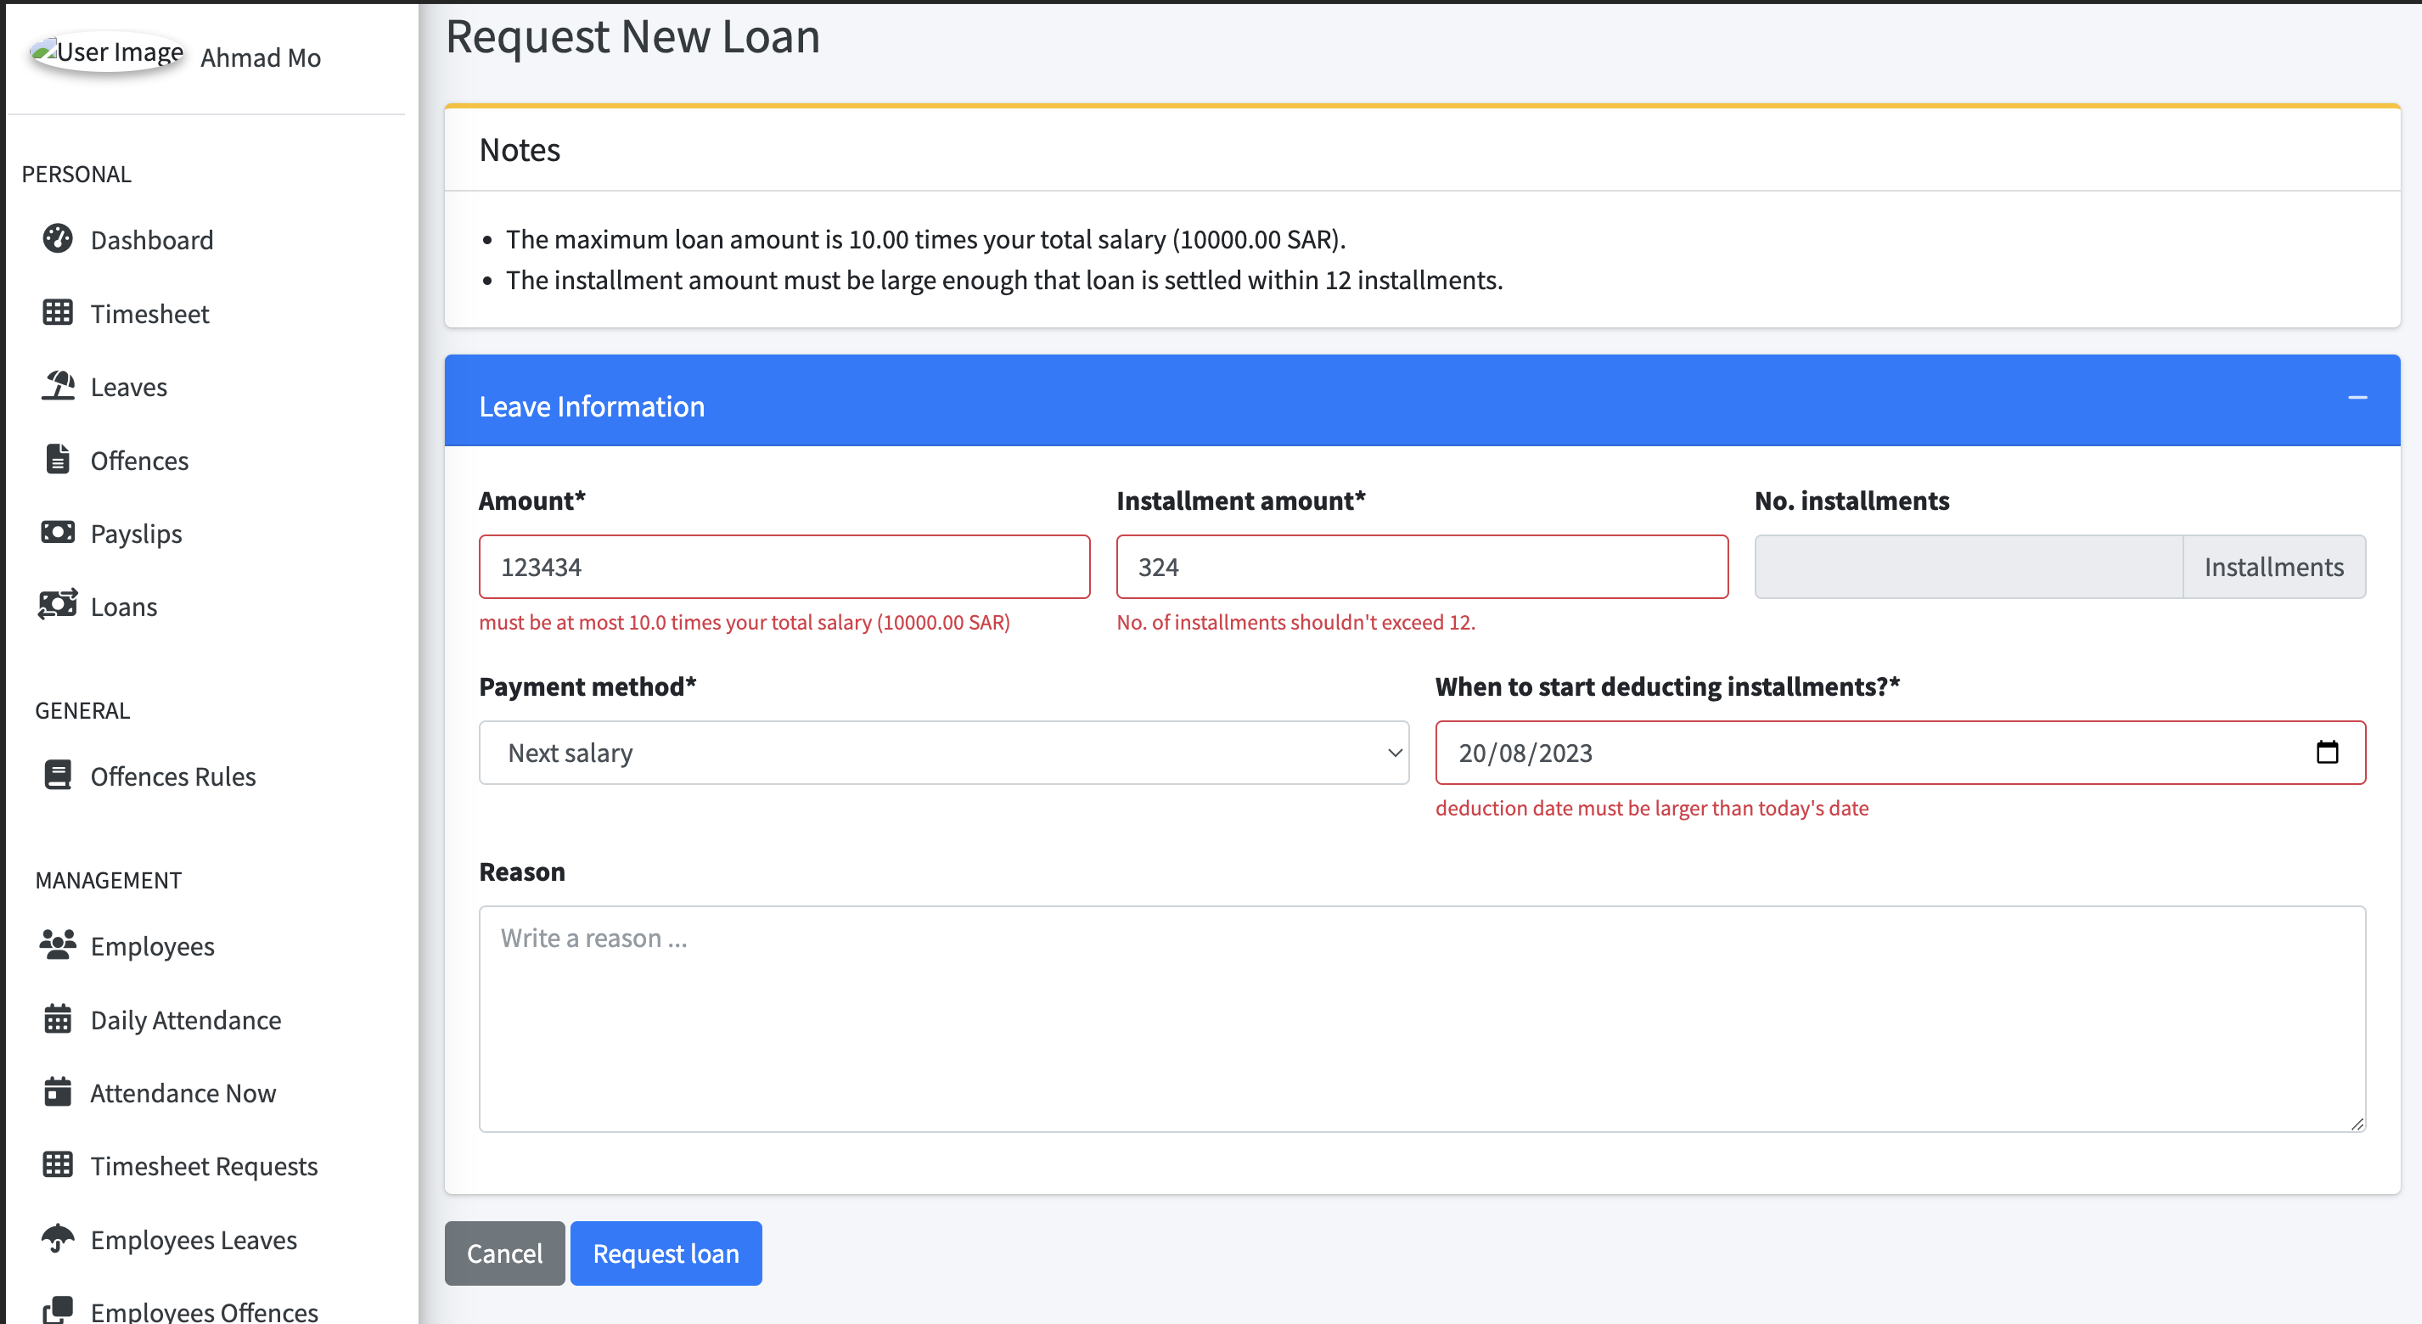
\includegraphics[width=0.7\textwidth]{figures/form-errors.png}
		\end{center}
		\caption{Request loan page, with some intentionally form errors.}
	\end{figure}
\end{frame}

\begin{frame}{Loans Feature}
	\begin{figure}
		\begin{center}
			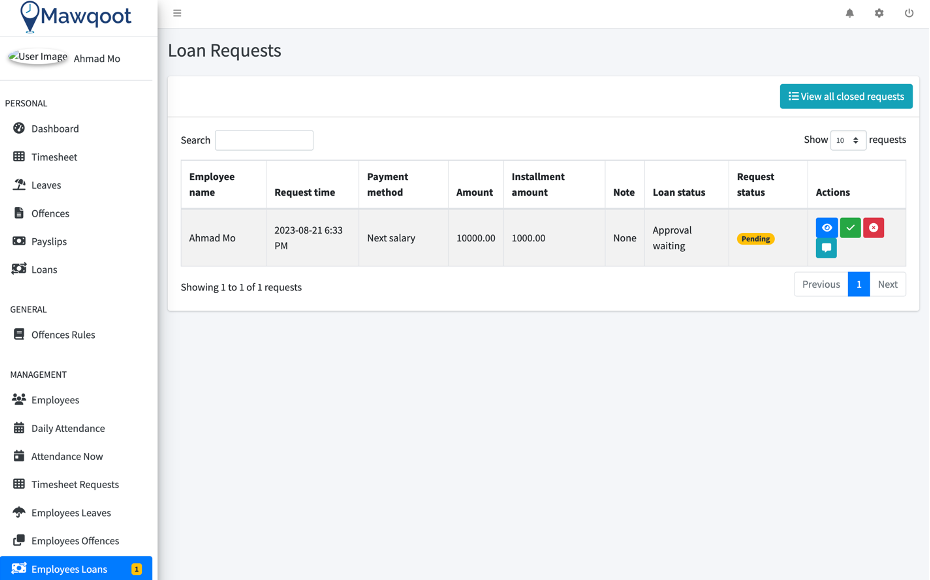
\includegraphics[width=0.6\textwidth]{figures/employees-loans.png}
		\end{center}
		\caption{Company admins can view all employees loans, Approve/Reject the request.}
	\end{figure}
\end{frame}

\begin{frame}{Loans Feature}
	\begin{figure}
		\begin{center}
			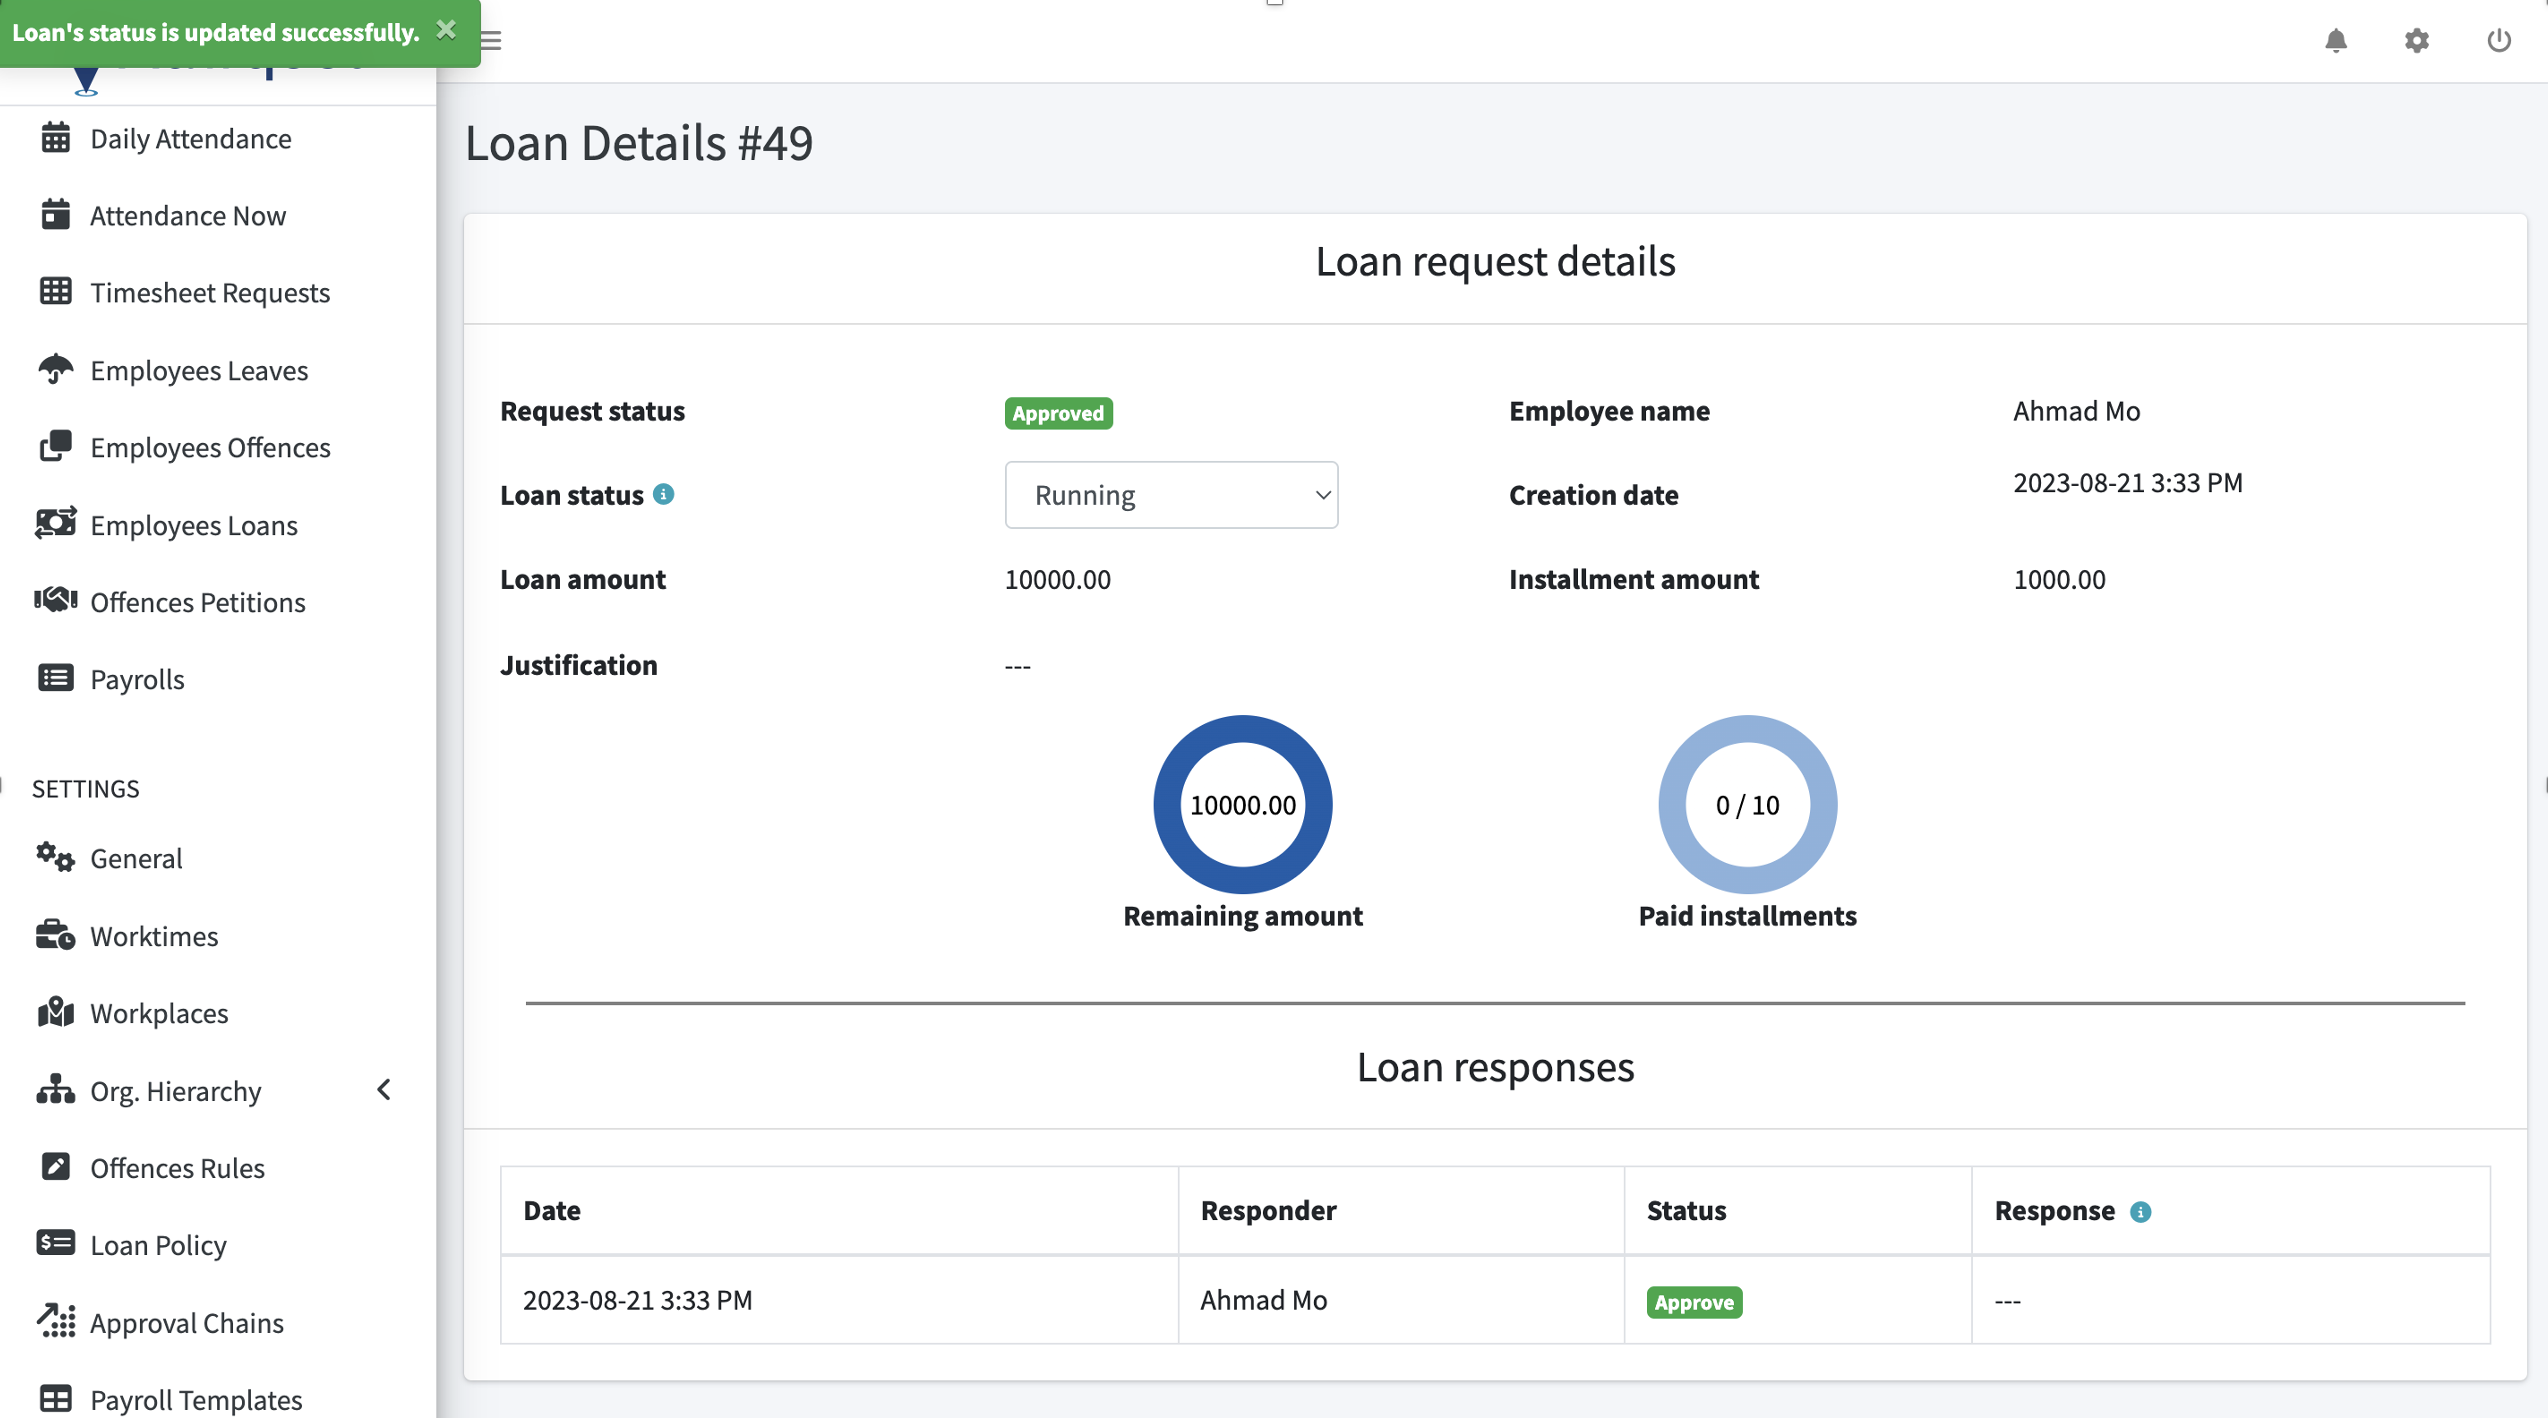
\includegraphics[width=0.6\textwidth]{figures/loan-details.png}
		\end{center}
		\caption{Loan page details. Current status. Accountants can change loan status.}
	\end{figure}
\end{frame}

\begin{frame}{Loans Feature}
	\begin{figure}
		\begin{center}
			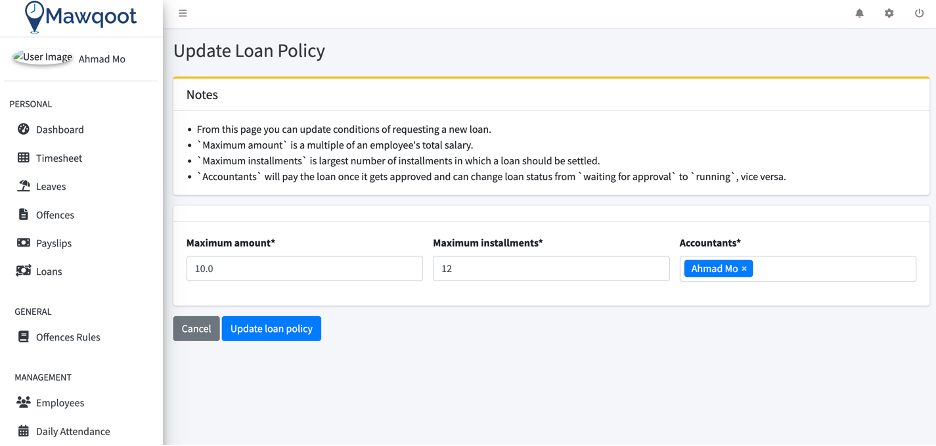
\includegraphics[width=0.75\textwidth]{figures/loan-policy.png}
		\end{center}
		\caption{Company's loan policy, it gets enforced while requesting new loan.}
	\end{figure}
\end{frame}


% --- Tools --- &
\section{Tools}

\begin{frame}
	\begin{figure}
		\begin{center}
			
\includegraphics[width=0.95\textwidth]{figures/frameworks.png}
		\end{center}
		\caption{Frameworks used by Mawqoot.}
	\end{figure}
\end{frame}

\begin{frame}
	\begin{figure}
		\begin{center}
			
\includegraphics[width=0.95\textwidth]{figures/tools-mng.png}
		\end{center}
		\caption{Management tools we used.}
	\end{figure}
\end{frame}

% --- Recommendation --- %
\section{Recommendation \& Conclusion}

\begin{frame}{Recommendation}
	Based on my experience during my summer training, I highly recommend working
	with the Mawqoot app, especially for students who want to gain practical
	experience in the software engineering field.
\end{frame}

\begin{frame}{Conclusion}
	This report outlines the most important skills I learned, the range of experience
	I obtained, and the personal and professional growth I experienced as a result of
	my summer training. Overall, this report aims to provide an accurate representation
	of my summer training experience, and I hope it serves as a valuable resource for those
	who may be interested in pursuing a career in the same field.
\end{frame}

% ---- The End ---- %

\begin{titleframe}{Thank you for listening!}
\end{titleframe}

\end{document}
